%LTeX: language=de-DE
\chapter{Einleitung}
Seit einigen Jahren findet man immer häufiger Bedienungen mit Touchscreens.
Ihr Einsatzbereich scheint keine Grenzen zu haben und so hat sich die Technologie in den letzten Jahren rasant weiterentwickelt.


\section{Ziel des Projekts}
In dieser Projektarbeit ist es Ziel, einen Sketch zu verfassen mit dem die Aufnahme von Koordinaten mittels eines resistiven Touchscreen umgesetzt werden kann.
Die aufgenommenen Daten werden anschließend nach der Wiederholbarkeit, der Linearität und der Auflösung untersucht.
Zum Schluss soll die Steuerung noch dahingehend erweitert werden, dass damit die Maus eines PCs gesteuert werden kann.


\section{Grundlagen}
\subsection{Resistives Touchscreen}
Es gibt bei den resistiven Touchscreens zwei unterschiedliche Gruppen.
Zum einen gibt es 4-Wire resistive Touchscreens.
Diese haben vier Anschlüsse, über die die Positionsauswertung läuft.
Zudem gibt es noch die 5-Wire resistive Touchscreens.
Hier sind fünf Anschlüsse, über die die Positionsauswertung durchgeführt wird.

Bei einem 4-Wire resistiven Touchscreen gibt es zwei Ebenen, bei denen die obere auf die untere gedrückt werden kann.
Eine Ebene ist mit Elektronen geladen und über die andere Ebene misst man die Spannung.
Für die andere Richtung ist es gespiegelt.
Über die unterschiedlichen Beträge der Spannung lässt sich dann die Koordinate in x-Richtung und y-Richtung bestimmen.

Die 5-Wire resistive Touchscreens haben ebenfalls zwei Ebene.
Der Unterschied zu den 4-Wire Touchscreen liegt darin, dass es nur eine Ebene gibt, die geladen ist.
Die obere Schicht misst  für x-Richtung und y-Richtung die abfallende Spannung.
Auch hier wird durch Druck auf die obere Schicht ein Kontakt zwischen den beiden Ebenen erstellt, damit die Messung durchgeführt werden kann.

Die 5-Wire Touchscreens sind gegenüber den 4-Wire widerstandsfähiger und haben dadurch eine längere Lebenserwartung \cite{5w4w}.

In diesem Projekt wird ein 4-Wire resistiver Touchscreen von der Firma Fujitsu verwendet.

Der verwendete Touchscreen besitzt für jede Richtung (x und y) jeweils zwei Anschlüsse.
\begin{figure}
    \centering
    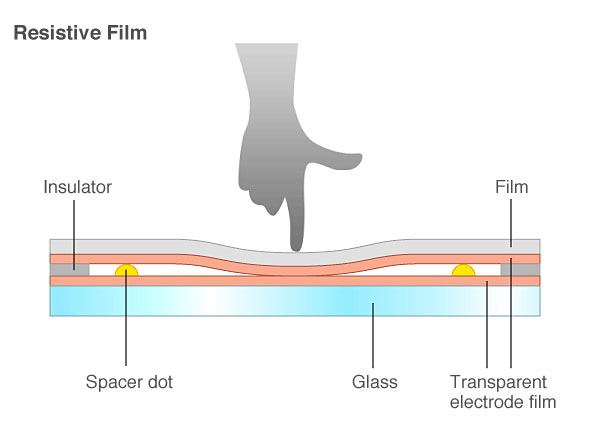
\includegraphics[width=0.6\linewidth]{fig/raster/4_wire_resistive_touch_screen.jpeg}
    \caption{Schemadarstellung eines 4-Wire resistiven Touchscreen \cite{4wschema}}
    \label{fig:4w}
\end{figure}
\subsection{Arduino Leonardo Board}
Die Steuerung des Touchscreens wird über das Arduino Leonardo Board realisiert. 
Dieses hat im Vergleich zum Arduino Uno Board die Möglichkeit sich als Peripherie an einem PC anzumelden.
Ermöglicht wird dies durch den Mikrocontroller ATmega32u4.
Der Mikrocontroller arbeitet nicht mit einem USB-Chip, sondern verarbeitet intern die serielle eingehende Daten und konvertiert diese für die Nutzung der USB-Schnittstelle.


%\section{Theorie}
% Um eine Koordinatenkomponente zu bestimmen, benötigt man drei Anschlüsse des Touchscreens.
% Zwei davon sind in der Richtung die man messen möchte und der dritte Anschluss ist einer der beiden übrigen Anschlüsse.
% Mit diesem wird der Spannungsteiler aufgespannt um den Wert der Koordinate zu bestimmen.

% In den \cref{fig:xylesen} auf \cref{fig:xylesen} wird dieser Lösungsansatz veranschaulicht.


% Um nun noch eine Messunsicherheiten aus zu filtern sollen, bei der Messung einer Koordinatenkomponente, mehrere Messpunkte aufgenommen werden.
% Diese werden anschließend über ein Filter-Funktion ausgewertet.
% Der Wert der bei der Auswertung als Ergebnis herauskommt, wird als gemessene Koordinatenkomponente ausgegeben.
% Das Schaltbild hierzu ist in \cref{fig:schaltbild} zu sehen.

% \begin{figure}[ht!]
%     \begin{subfigure}{0.49\textwidth}
%         \centering
%         %\includesvg[width=\textwidth]{fig/schematics/sch_read_x}
%         \caption{in x-Richtung.}
%         \label{fig:xlesen}
%     \end{subfigure}
%     \hfill
%     \begin{subfigure}{0.49\textwidth}
%         \centering
%         %\includesvg[width=\textwidth]{fig/schematics/sch_read_y}
%         \caption{in y-Richtung.}
%         \label{fig:ylesen}
%     \end{subfigure}
%     \caption{Schaltbild für das Messen der Koordinatenpunkte}
%     \label{fig:xylesen}
% \end{figure}
% \begin{figure}[ht!]
%     \centering
%     %\includesvg[width=\textwidth]{fig/schematics/sch_full}
%     \caption{Schaltbild des Projekts.}
%     \label{fig:schaltbild}
% \end{figure}
% Die einzelne Lösungsansätze werden in der Arduino-Umgebung umgesetzt.
% Der Programmablauf ist in \cref{fig:flowchart} als Flow-Chart dargestellt.

% \begin{figure}
%     \centering
%     %\includesvg[height=0.4\textheight]{fig/flowchart/flow_chart}
%     \caption{Darstellung des Programmablaufs.}
%     \label{fig:flowchart}
% \end{figure}